 \documentclass[11pt]{article}
% \pagestyle{empty}
\usepackage{mathtools}
\DeclarePairedDelimiter\ceil{\lceil}{\rceil}
\DeclarePairedDelimiter\floor{\lfloor}{\rfloor}
\usepackage{algorithmicx}
\usepackage{algpseudocode}
\usepackage{algorithm}
\usepackage[makeroom]{cancel}

\usepackage[letterpaper, portrait, margin=1in]{geometry}
\usepackage{epsf}
\usepackage{pseudocode}
% \usepackage{times}
% \usepackage{mathptm}

\def\O{\mathop{\smash{O}}\nolimits}
\def\o{\mathop{\smash{o}}\nolimits}
\newcommand{\e}{{\rm e}}
\newcommand{\R}{{\bf R}}
\newcommand{\Z}{{\bf Z}}

\title{CS 124, Problem Set 5}
\author{Jessica Wang}
\date{April 1, 2016}

\begin{document}
\maketitle
\section*{Problem 1}
\paragraph{A)}
\begin{align*}
p(different) &= 1\times (1-\frac{1}{n}) \times (1-\frac{2}{n}) \times ... \times (1-\frac{c_1\sqrt{n}}{n})\\
\text{Using Taylors Approx: }&1-x = e^{-x}\\
p(different) &= 1\times e^{-\frac{1}{n}} \times e^{-\frac{2}{n}} \times ... \times e^{-\frac{c_1\sqrt{n}}{n}}\\
&= 1 \times e^{\frac{-(1+2+...+c_2\sqrt{n})}{n}}\\
&=1 \times e^{\frac{-(c_1\sqrt{n}(c_1\sqrt{n}+1))}{2n}}\\
&= e^{\frac{-c_1^2}{2} - \frac{c_1}{2\sqrt{n}}}\\
&= e^{\frac{-c_1^2}{2}} \text{  for large }n\\
e^{-1} &= e^{\frac{-c_1^2}{2}}\\
-1 &= \frac{-c_1^2}{2}\\
c_1&=\sqrt{2}
\end{align*}
\paragraph{B)}
\begin{align*}
p(different) &= 1\times (1-\frac{1}{n}) \times (1-\frac{2}{n}) \times ... \times (1-\frac{c_1\sqrt{n}}{n})\\
\text{Using Taylors Approx: }&1-x = e^{-x-x^2}\text{  when x }\leq \frac{1}{2}
\end{align*}
\begin{align*}
e^{-(\frac{c_2\sqrt{n}(c_2\sqrt{n}+1)}{2n} + \frac{c_2\sqrt{n}(c_2\sqrt{n}+1)(2c_2\sqrt{n}+1)}{6n^2})} &\geq \frac{1}{2}\\
-(\frac{c_2\sqrt{n}(c_2\sqrt{n}+1)}{2n} + \frac{c_2\sqrt{n}(c_2\sqrt{n}+1)(2c_2\sqrt{n}+1)}{6n^2}) &\geq \ln{\frac{1}{2}}\\
\frac{c_2\sqrt{n}(c_2\sqrt{n}+1)}{2n} + \frac{c_2\sqrt{n}(c_2\sqrt{n}+1)(2c_2\sqrt{n}+1)}{6n^2} &\geq \ln{2}\\
\frac{c_2\sqrt{n}(c_2\sqrt{n}+1)}{2n} + \cancelto{0}{\frac{c_2\sqrt{n}(c_2\sqrt{n}+1)(2c_2\sqrt{n}+1)}{6n^2}} &\geq \ln{2}\\
\frac{c_2^2n}{2n} + \cancelto{0}{\frac{c_2\sqrt{n}}{2n}} &\geq \ln{2}\\
\frac{c_2^2}{2} &= \ln{2}\\
c_2&=\sqrt{2 \ln{2}}
\end{align*}

\section*{Problem 2}
\subsection*{Part a}
Consider two hash functions each of which cooresponds to 26 bits. The first hash function will change the bit that corresponds to the first letter of the word being hashed and the second has function will change the bit that corresponds to the last letter of the word being hashed. If we input the words $austin$ and $apple$ into the function then try to remove $apple$, we will also remove the mark for first letter $a$ completely, meaning that it would indicate that $austin$ was never inputted. 

\subsection*{Part b}
Within a specific counter, there are $\frac{m}{k}$ possible counters within the table corresponding to this hash function. Since the hash function is suppose to be truely random there is a $\frac{1}{\frac{m}{k}}$ that a counter will be increased. Overflow will occur when a counter is increased for the 16th time because the 4 bits can only hold the values 0-15. The probability of a counter increasing $n$ times can be represented by a binomial distribution $X \sim Bin(n, \frac{1}{\frac{m}{k}})$. To find the probabilty of overflow find $Pr(X \geq 2^4 = 16) = 1-Pr(X = 15)- Pr(X=14) - .... - Pr(X =1) - Pr(X=0) = 1 -  \sum_{i=0}^{15} {n \choose i}(\frac{1}{\frac{m}{k}})^i(1-\frac{1}{\frac{m}{k}})^{n-i}$. \\

Calculating the probabilty when $k=(m/n)*ln2$ simply involves substituation. Therefore $1 -  \sum_{i=0}^{15} {n \choose i}(\frac{1}{\frac{m}{k}})^i(1-\frac{1}{\frac{m}{k}})^{n-i} = 1 -  \sum_{i=0}^{15} {n \choose i}(\frac{1}{\frac{m}{m/n*ln2}})^i(1-\frac{1}{\frac{m}{m/n*ln2}})^{n-i} = 1 -  \sum_{i=0}^{15} {n \choose i}(\frac{n}{ln2})^i(1-\frac{n}{ln2})^{n-i}$
\subsection*{Part c}
The Counting Bloom would have the same false postive probabilty as the standard Bloom filter. This is because when hashing the same bits/counters will be updated (either changed to one or increased in counter). Thus when hashing elements the same same bits/counters will shown that the spot has been visited. Therefore the chance of a false positive occuring is the same in both standard Bloom filters and Counting Bloom filters because the same bits/counters will be marked as visited, indicating a false positive. This false positive is $(1-e^{-nh/m})^h$

\section*{Problem 3}
It is safe to assume that this match will only occur once because the hashing is saved as a 64 bit, giving a $2^{64}$ possible hashings. Because hashings are truly random there is a $1/2^{64}$ chance of two distinct elements getting the same hashing for a super-sketch. This number is extremely low making it safe to assume that it will not happen. \\

With resemblance $r$ there is an $r^{14}$ change of a super sketch matching because there is 14 values in the sketch. Therefore the probability of many sketchs matching can be modeled by a binomial distribution $X \sim Bin(6,r^{14})$. Thus the change of two or more sketches matching is $Pr(X \geq 2) = 1 - Pr(X=0) - Pr(X=1) =1 - {6 \choose 0}(r^{14})^0(1-r^{14})^6 - {6 \choose 1})(r^{14})^1(1-r^{14})^5 = 1*1*(1-r^{14})^6 - 6*r^{14}(1-r^{14})^5$\\

The graph of this equation looks like \\

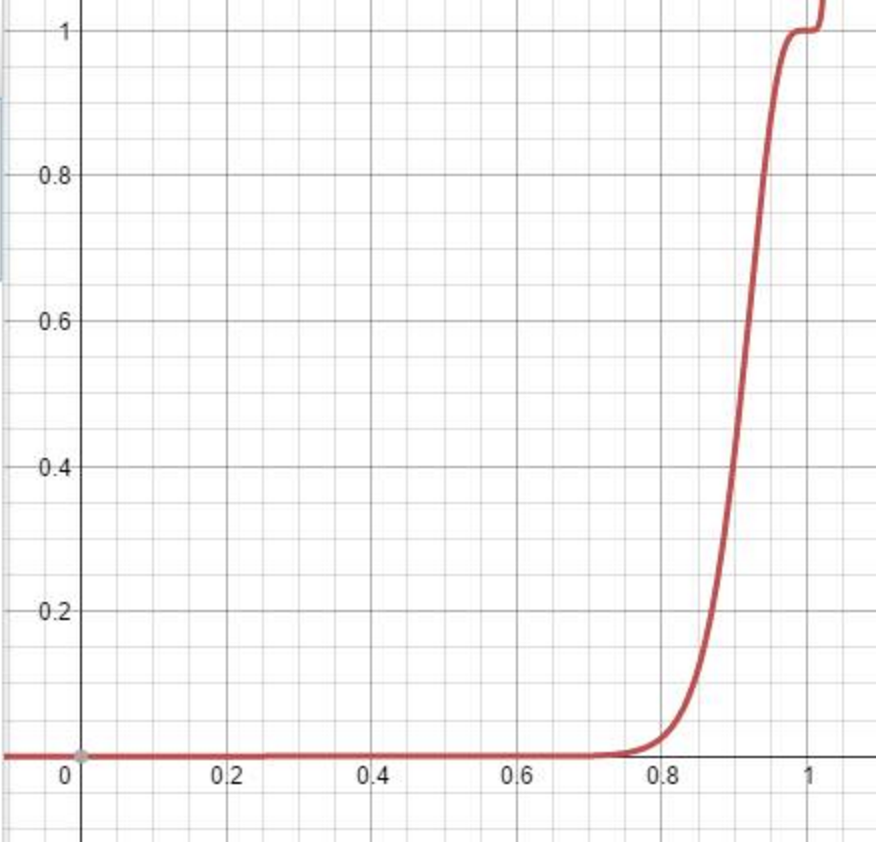
\includegraphics[scale=.75]{graph.png} \\
This indicates that there is little chance of two or more super sketches matching until .75 when the chance steeply increases until .9 when it is almost a guarentee that at least two super matches will occur

Using only a 16 bit or 8 bit hash will only give $2^{16}$ or $2^8$ possible different hash values. Therefore there is a much higher probability that distinct 14 values will hash to the same values. This would create many more false positives and prevent you from properly 

\section*{Problem 4}
The fingerprinting pattern-matching scheme can be generalized for a matrix by iterated through the $n$ rows of the text matrix seaching for the first row of the pattern matrix. When the first row of the pattern matrix is found then it would indicate an index that the pattern matrix would be found at.  Each of these rows would utilize the one dimensional fingerprinting pattern matching as described in class. Thus this would require $n$ pattern matchings. Repeat this with every row of the pattern matrix to find where each row of the pattern matrix appears in the text matrix. Let $S_{ij,}$ be the $m$-sized subsring in row $i$ and column $j$. If $S_{i,j}$ has the same fingerprint as the first row of the small matrix and $S_{i+1,j}$ has the same fingerprint as the second row and etc. then we have an $m$x$m$ matrix who has the same fingerprint as the pattern matrix and we can check this matrix elementwise to ensure that it matches the pattern matrix. We can optimize this slightly by only checking against the first 3 rows of the pattern matrix. While this will increase the number of matricies we have the check elementwise it will reduce the time it takes to fingerprint. \\

For each row of pattern matrix searched it will take $O(n^2)$ space to store the fingerprints ($n^2$ space for each row checked for $3n^2$ space over all). It takes $3n^2$ time to check a row of the pattern matrix against all the rows of the text matrix. Matching the fingerprints to the fingerprints of the first three rows of the pattern matrix will take $3n^2$ time to have time complexity.  $O(n^2)$ On average there will be $n^2/p^3$ matrices to check elementwise, so overall checking elementwise will take $O(m^2n^2/p^3)$ time. Overall the algorithm will take $O(n^2+m^2n^2/p^3$ time.

\section*{Problem 5}
To find the witness I utilized the Miller-Rabin primality test which indicates whether a number $n$ is prime. It halts when it determines $n$ is found to be composite according to Fermat's Little Theorem and by printing the value that causes Fermat's Little Theorem to be false we can find a witness. 

The psuedocode is below:
\begin{algorithmic}
\Function {EvenFactor}{$num$}
	\State $num --$
	\State $count = 0$
	\While{$num$ is even} 
		\State $num= num/2$
		\State $count++$	
	\EndWhile
\EndFunction

\Function{ChooseRandom}{$num$}
	\State $a$ = random number from 2 to $num -2$
	\If { $a$ is factor of $n$}
		\State ChooseRandom($num$)
	\Else
		\State return $a$
	\EndIf
\EndFunction

\Function {MillerRabin}{n, k}
	\State r,d = EvenFactor(n)
	\For {$x$ from 0 to $k$}
		\State $a$ = ChooseRandom(n)
		\State x = $a^d$ (mod $n$)
		\If {$x$=1 or $x = n$-1}
			continue MillerRabin
		\EndIf
		\For {$i$ from 1 to $r-1$}
			\State $x = x^2 (mod n)$
			\If $x =1$
				\State return "composite with witness $a$"
			\EndIf
			\If {x = n-1}
				\State continue MillerRabin
			\EndIf
		\EndFor
		\State return "Composite"
	\EndFor
	\State return "Probably Prime"
\EndFunction
\end{algorithmic}

Running this code allowed me to find witness 558888. We can prove this is a witness by calculating $558888^{636127-1} \equiv 318448$ (mod $636127$) which contradicts Fermat's Little Theorem. \\

To deal with Carmichael numbers we add a few lines of code to our Rabin Miller Function:

\begin{algorithmic}
\Function {MillerRabin}{n, k, carmichael = True}
	\State r,d = EvenFactor(n)
	\For {$x$ from 0 to $k$}
		\State $a$ = ChooseRandom(n)
		\State x = $a^d$ (mod $n$)
		\If {$x$=1 or $x = n$-1}
			continue MillerRabin
		\EndIf
		\For {$i$ from 1 to $r-1$}
			\State $x = x^2 (mod n)$
			\If $x =1$
				\State return "composite with witness $a$, $u$ value $i$ and even factor $r$"
			\EndIf
			\If {x = n-1}
				\State continue MillerRabin
			\EndIf
		\EndFor
		\If {carmichael}
			\State continue
		\Else
			\State return "Composite"
		\EndIf
	\EndFor
	\State return "Probably Prime"
\EndFunction
\end{algorithmic}


This will allow the function to return the witness and the $u$ value such that $a^{2^u*r} \not\equiv \pm 1 $ (mod $n$) and $a^{2^{u+1}*r} \equiv 1$ (mod $n$), which means despite $a^{n-i} \equiv 1$ (mod $n$) $n$ is still not prime. The code returned the witness 77564 with a $u$ value of 0 and a $r$ value of 36801.

\section*{Problem 6}
To find the RSA first the code read in the string and created an array that saved the ascii value of each character in an array. Next if would enumerate overe this array and save each value as an 8 bit number. Next it would join all these numbers in the array into a single value and save it as $message$.

Next it would calculate let the first number in the key be $n$ and the second be $e$. The code could calculate $mesage^e$ (mod $n$) which is your encoded message. This is 27016764340118192395712492378.
\end{document}





